\documentclass[11pt]{article}

% ======================= PAQUETES =======================
\usepackage[utf8]{inputenc}
\usepackage[T1]{fontenc}
\usepackage[spanish,es-tabla]{babel}
\usepackage{geometry}
\geometry{a4paper, top=2.8cm, bottom=2.8cm, left=2.6cm, right=2.6cm}

\usepackage{titlesec}
\usepackage{fancyhdr}
\usepackage{booktabs}
\usepackage{array}
\usepackage{enumitem}
\usepackage[table]{xcolor}
\usepackage{tcolorbox}
\usepackage{graphicx}
\usepackage{hyperref}
\usepackage{tikz}
\usetikzlibrary{arrows.meta, positioning, shapes.geometric}
\usepackage{parskip}
\usepackage{caption}

% ======================= COLORES =======================
\definecolor{primaryblue}{RGB}{28,58,92}
\definecolor{accentblue}{RGB}{47,109,161}
\definecolor{lightgray}{RGB}{245,246,248}
\definecolor{midgray}{RGB}{110,110,110}

% ======================= TÍTULOS DE SECCIÓN =======================
\titleformat{\section}
  {\Large\bfseries\color{primaryblue}}
  {\thesection.}{0.4em}{}
\titlespacing*{\section}{0pt}{1.6em}{0.8em}

\titleformat{\subsection}
  {\large\bfseries\color{accentblue}}
  {\thesubsection}{0.4em}{}
\titlespacing*{\subsection}{0pt}{1.2em}{0.6em}

% ======================= ENCABEZADO / PIE =======================
\pagestyle{fancy}
\fancyhf{}
\renewcommand{\headrulewidth}{0.4pt}
\renewcommand{\footrulewidth}{0pt}
\fancyhead[L]{\small\color{midgray} Recomendación local de citas académicas}
\fancyhead[R]{\small\color{midgray} Semana 3 -- Reporte de avance}
\fancyfoot[C]{\small\color{midgray} \thepage}

% ======================= HYPERREF =======================
\hypersetup{
  colorlinks=true,
  linkcolor=accentblue,
  citecolor=accentblue,
  urlcolor=accentblue,
  pdftitle={Recomendación local de citas académicas mediante aprendizaje automático},
  pdfauthor={Maestría en Inteligencia Artificial - Universidad de los Andes}
}

\newcommand{\notabox}[1]{%
  \begin{tcolorbox}[colback=lightgray, colframe=accentblue, boxrule=0.6pt,
    left=8pt, right=8pt, top=6pt, bottom=6pt, arc=2pt]
    \small #1
  \end{tcolorbox}
}

\begin{document}

% ======================= PORTADA =======================
\begin{titlepage}
\centering
\vspace*{2.5cm}

{\Large \color{midgray} Maestría en Inteligencia Artificial}\\[0.2cm]
{\large \color{midgray} Universidad de los Andes}\\[2.5cm]

{\color{primaryblue}\rule{\linewidth}{1.2pt}}\\[0.6cm]
{\Huge \bfseries \color{primaryblue} Recomendación local de citas\\ académicas mediante aprendizaje\\ automático}\\[0.6cm]
{\color{primaryblue}\rule{\linewidth}{1.2pt}}\\[0.8cm]

{\Large Reporte de avance del microproyecto -- Semana 3}\\[3cm]

\begin{tabular}{rl}
\textbf{Nombres participantes:} & Carlos Duque, Carlos Caicedo, Jose Zambrana, John Arias \\[4pt]
\textbf{Proyecto:} & Desarrollo de Soluciones \\[4pt]
\textbf{Docente:} & Juan Fernando Pérez \\[4pt]
\textbf{Fecha:} & 23 de agosto de 2026 \\
\end{tabular}

\vfill
{\small \color{midgray} Universidad de los Andes -- Maestría en Inteligencia Artificial}
\end{titlepage}

\tableofcontents
\newpage

% ======================= 1. PROBLEMA Y CONTEXTO =======================
\section{Problema y contexto}

El crecimiento sostenido de la literatura científica dificulta que investigadores, estudiantes y autores identifiquen con rapidez los trabajos más pertinentes para respaldar una afirmación mientras redactan un documento académico. La búsqueda manual de referencias implica formular consultas, revisar resultados y determinar posteriormente cuáles documentos guardan una relación directa con el fragmento específico que se está escribiendo.

La recomendación local de citas aborda este problema utilizando como consulta el contexto textual próximo al lugar donde se requiere una referencia. A partir de ese fragmento, el sistema busca y ordena artículos candidatos que podrían ser citados. Esta formulación corresponde al problema de \textit{local citation recommendation} descrito por Gu, Gao y Hahnloser (2022), en el cual una referencia faltante se recomienda a partir del contexto local de cita.

El microproyecto propone desarrollar un prototipo que reciba como entrada un contexto académico en inglés y produzca un ranking de artículos candidatos. El objetivo es apoyar la etapa inicial de búsqueda de referencias, sin reemplazar la revisión crítica del artículo ni la decisión final del autor sobre qué fuente citar.

\subsection{Usuario objetivo}

El usuario objetivo es una persona que se encuentre redactando o revisando literatura académica. Entre los usuarios potenciales se consideran investigadores, estudiantes universitarios, estudiantes de posgrado y autores de artículos científicos. El sistema se plantea como una herramienta de apoyo para reducir el esfuerzo de búsqueda inicial y facilitar la identificación de literatura potencialmente pertinente.

% ======================= 2. PREGUNTA DE NEGOCIO Y ALCANCE =======================
\section{Pregunta de negocio y alcance del proyecto}

\notabox{¿Cómo apoyar a un autor de textos académicos en la identificación de artículos potencialmente relevantes para citar, utilizando el contexto textual local en el que requiere incluir una referencia?}

Desde una perspectiva analítica, esta pregunta se traduce en: ¿es posible utilizar un modelo supervisado para estimar la relevancia de diferentes artículos académicos respecto a un contexto local de cita y ordenar los candidatos de acuerdo con dicha relevancia?

\subsection{Alcance del proyecto}

El microproyecto desarrollará un prototipo funcional de recomendación local de citas académicas. La entrada principal será un fragmento de texto académico en inglés correspondiente al contexto donde se requiere una cita. Para cada contexto, el sistema evaluará artículos candidatos, calculará un puntaje de relevancia y presentará al usuario las recomendaciones mejor posicionadas.

\subsubsection{Dentro del alcance}
\begin{itemize}[leftmargin=1.4em, itemsep=2pt]
  \item Procesamiento de contextos locales de cita.
  \item Procesamiento de la información de los artículos candidatos, principalmente título y resumen.
  \item Construcción de ejemplos supervisados positivos y negativos.
  \item Entrenamiento y comparación de modelos para estimar la relevancia de un artículo frente a un contexto.
  \item Generación de un ranking de artículos candidatos.
  \item Construcción posterior de una API para servir las inferencias del modelo.
  \item Construcción de un tablero interactivo para consumir la API y visualizar resultados y datos relevantes.
  \item Empaquetamiento de los componentes para su despliegue mediante contenedores Docker.
\end{itemize}

\subsubsection{Fuera del alcance}
Para mantener un alcance compatible con las ocho semanas del curso, se excluyen de este microproyecto:
\begin{itemize}[leftmargin=1.4em, itemsep=2pt]
  \item La clasificación de las nueve funciones discursivas de cita.
  \item La anotación humana de dichas funciones.
  \item La construcción de un corpus de miles de ejemplos por categoría.
  \item La recuperación de párrafos completos del artículo citado.
  \item La comparación extensa con modelos comerciales de lenguaje.
\end{itemize}
Estas actividades se reservan para el proyecto de grado.

\subsection{Formulación del problema de aprendizaje automático}

El problema de recomendación se transformará inicialmente en una tarea supervisada de clasificación de relevancia. Para cada contexto de cita se construirán ejemplos positivos y negativos:

\begin{itemize}[leftmargin=1.4em, itemsep=3pt]
  \item \textbf{Ejemplo positivo:} contexto de cita + artículo realmente citado $\rightarrow$ relevante (1).
  \item \textbf{Ejemplo negativo:} contexto de cita + artículo candidato no citado $\rightarrow$ no relevante (0).
\end{itemize}

El modelo estimará la relevancia de un artículo candidato condicionado al contexto de cita. Durante la inferencia, se evaluarán varios candidatos y se ordenarán según el puntaje estimado. Los artículos con mayor puntuación serán presentados como recomendaciones.

\subsection{Enfoque predictivo y resultado esperado}

Como línea base se utilizará una representación TF--IDF con similitud coseno. Posteriormente se evaluará un modelo supervisado, inicialmente una regresión logística o un clasificador lineal, con características derivadas de la relación entre el contexto y el título y resumen del artículo candidato. Si los recursos lo permiten, se evaluarán \textit{embeddings} de textos científicos.

Para cada contexto de entrada, el sistema devolverá una lista ordenada de artículos con un puntaje de relevancia, tal como se ilustra en la maqueta del prototipo (Figura~\ref{fig:mockup}).

% ======================= 3. CONJUNTOS DE DATOS =======================
\section{Conjuntos de datos a emplear}

El conjunto de datos base proviene del repositorio \textit{Local-Citation-Recommendation}, publicado como código complementario del trabajo de Gu et al. (2022). El repositorio incluye un conjunto denominado \texttt{custom} que corresponde a ACL-200 y muestra la estructura requerida para entrenar y evaluar un sistema de recomendación local de citas (Gu, 2022).

Para el desarrollo inicial se utilizarán cinco componentes:

\begin{itemize}[leftmargin=1.4em, itemsep=3pt]
  \item \texttt{contexts.json}: contiene los contextos locales de cita e información como \texttt{masked\_text}, \texttt{context\_id}, \texttt{citing\_id} y \texttt{refid}.
  \item \texttt{papers.json}: contiene la base de artículos y su información textual, principalmente título y \textit{abstract}.
  \item \texttt{train.json}: contiene los ejemplos destinados al entrenamiento.
  \item \texttt{val.json}: contiene los ejemplos destinados a validación.
  \item \texttt{test.json}: contiene los ejemplos destinados a evaluación.
\end{itemize}

En los conjuntos de entrenamiento, validación y prueba, \texttt{positive\_ids} identifica el artículo realmente citado por el contexto y constituye la referencia para construir el problema supervisado. La Sección~\ref{sec:eda} presenta el perfilamiento cuantitativo y las comprobaciones de calidad realizadas sobre estos archivos.

% ======================= 4. REPOSITORIO GIT =======================
\section{Repositorio Git usado para el código}

El código del proyecto se versiona mediante Git y se aloja en el siguiente repositorio:

\begin{center}
\url{https://github.com/Byron971/microproyecto-local-citation}
\end{center}

En este repositorio se registran los cambios asociados al preprocesamiento de datos, la construcción de los ejemplos supervisados, el entrenamiento de los modelos y, en etapas posteriores, el desarrollo de la API y el tablero interactivo.

% ======================= 5. REPOSITORIO DVC =======================
\section{Repositorio DVC en uso para los datos}

Dado el tamaño de los archivos de datos (\texttt{contexts.json}, \texttt{papers.json}, \texttt{train.json}, \texttt{val.json}, \texttt{test.json}), su versionamiento se gestiona mediante DVC (\textit{Data Version Control}), utilizando un bucket de Amazon S3 como almacenamiento remoto. Esto permite mantener el historial de versiones de los datos de forma separada del repositorio de código, evitando incrementar su tamaño y facilitando la reproducibilidad de los experimentos.

Las Figuras~\ref{fig:dvc1} y~\ref{fig:dvc2} muestran el proceso de inicialización de DVC y la carga de los datos al repositorio remoto en S3.

\begin{figure}[h!]
\centering
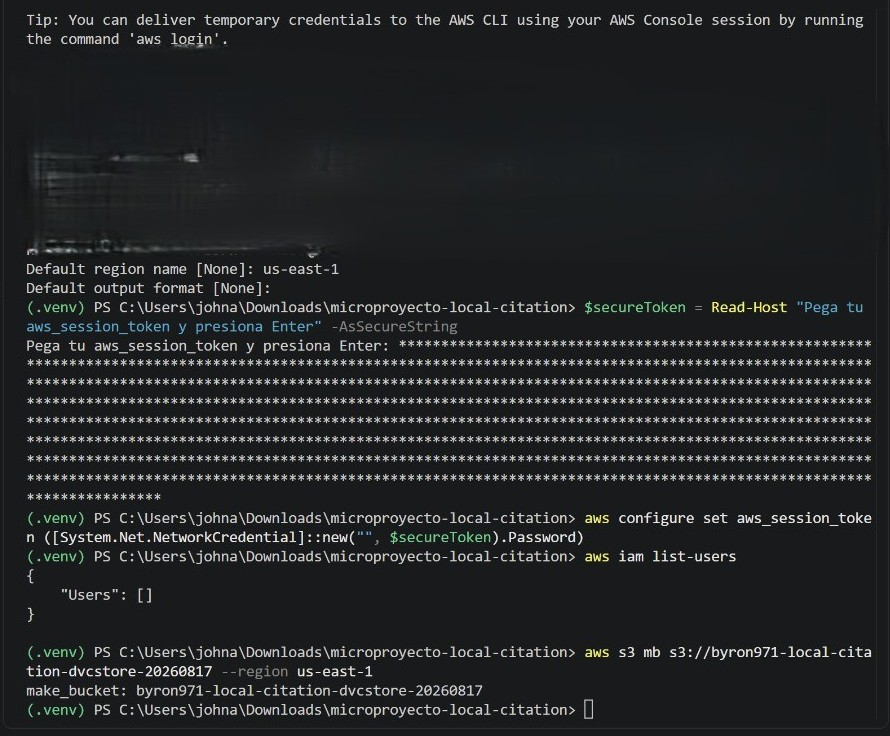
\includegraphics[width=0.68\textwidth]{buckets3.jpeg}
\caption{Creación exitosa de bucket en S3}
\label{fig:dvc1}
\end{figure}

\begin{figure}[h!]
\centering
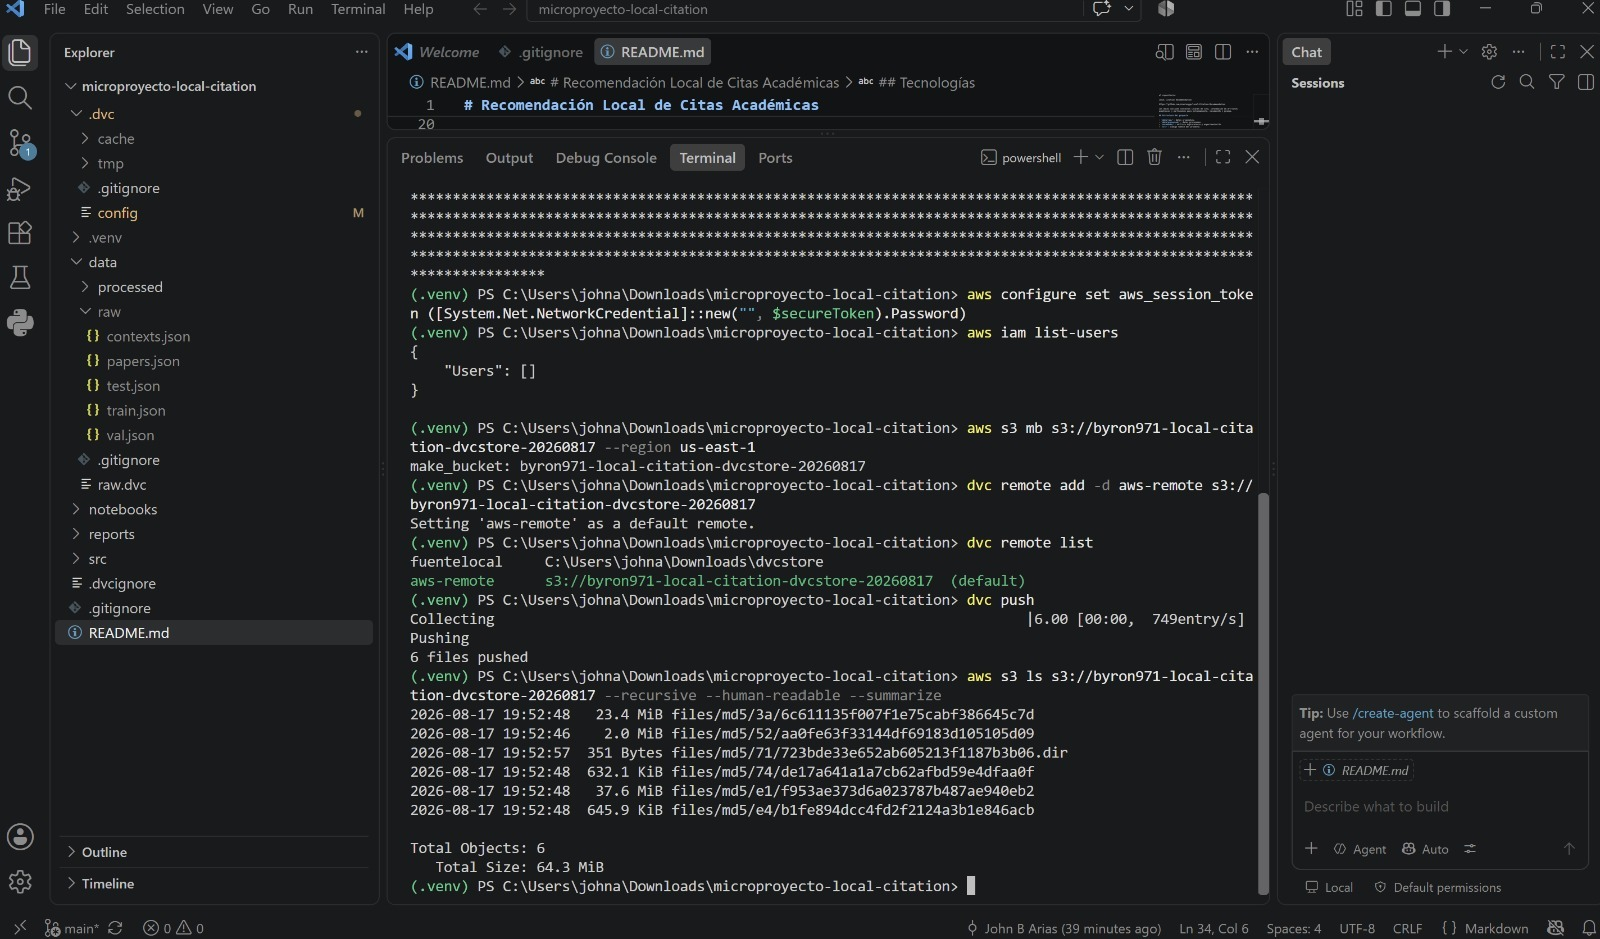
\includegraphics[width=0.68\textwidth]{creaciondvcs3.jpeg}
\caption{Proceso de carga (\textit{push}) de los datos versionados al repositorio DVC en S3}
\label{fig:dvc2}
\end{figure}
% ======================= 6. EXPLORACION DE DATOS =======================
\section{Exploración de los datos}
\label{sec:eda}

La exploración se realizó en el notebook \texttt{notebooks/01\_exploracion\_datos.ipynb} sobre la versión de los datos registrada con DVC. El corpus contiene 63.768 contextos y 19.776 artículos candidatos. De los contextos, 49.356 forman consultas supervisadas: 30.390 de entrenamiento, 9.381 de validación y 9.585 de prueba (Figura~\ref{fig:eda-particiones}); los 14.412 restantes no pertenecen a estas particiones y no se utilizarán para evaluar el modelo.

\begin{figure}[h!]
\centering
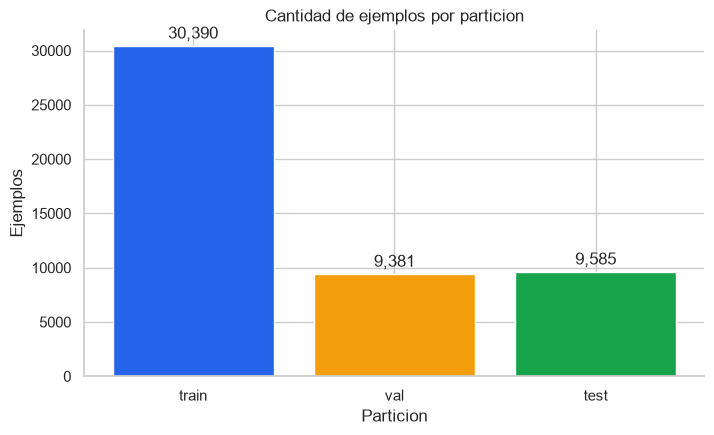
\includegraphics[width=0.58\textwidth]{eda_particiones.png}
\caption{Cantidad de consultas en las particiones de entrenamiento, validación y prueba.}
\label{fig:eda-particiones}
\end{figure}

\subsection{Calidad e integridad}

Las relaciones entre archivos son consistentes: no hay contextos referenciados ni artículos citados inexistentes; tampoco hay títulos o resúmenes vacíos. Todas las consultas contienen un único \texttt{positive\_id}, este coincide con \texttt{refid}, y cada contexto contiene exactamente un marcador \texttt{TARGETCIT}. Se identificaron 1.705 textos de contexto duplicados, equivalentes al 2,7\% de los 63.768 contextos, por lo que deberá evitarse que una repetición influya de manera desproporcionada en el entrenamiento.

La separación de datos respeta el aislamiento exigido en la propuesta: no se encontraron documentos citantes compartidos ni pares citante--citado repetidos entre \textit{train}, \textit{validation} y \textit{test}. Esta comprobación reduce el riesgo de fuga de información y hace más confiable la evaluación posterior.

\subsection{Longitud de los textos}

El contexto tiene una mediana de 63 palabras y un percentil 95 de 72; el máximo observado es 153. Los títulos tienen una mediana de 8 palabras, mientras que los resúmenes presentan una mediana de 106 y un percentil 95 de 465 palabras. La cola larga de los resúmenes, visible en la Figura~\ref{fig:eda-longitudes}, obliga a definir y medir una estrategia de truncamiento al preparar entradas para SciBERT.

\begin{figure}[h!]
\centering
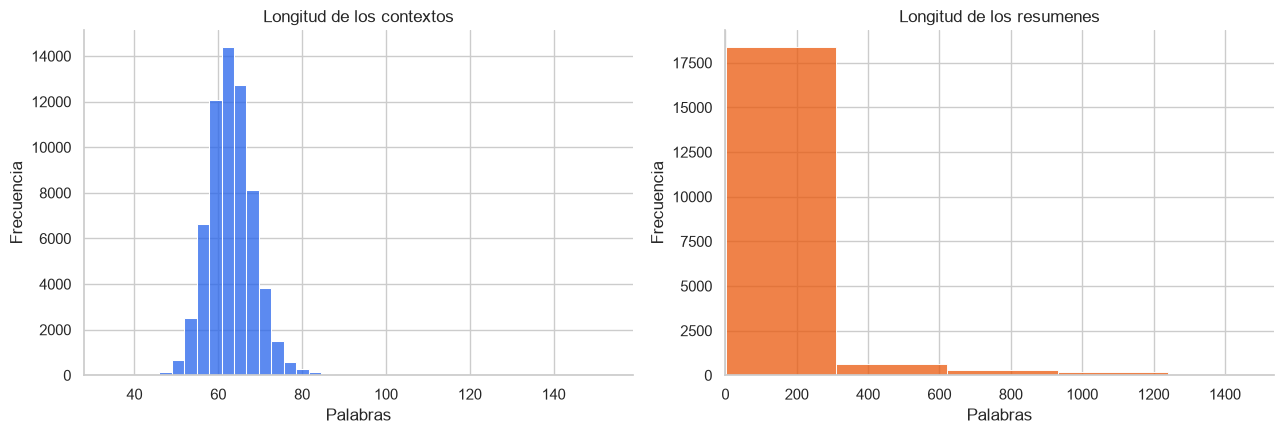
\includegraphics[width=0.84\textwidth]{eda_longitudes.png}
\caption{Distribución de la longitud de los contextos y resúmenes, medida en palabras. En los resúmenes se muestra hasta el percentil 99 para evitar que los valores extremos oculten la distribución principal.}
\label{fig:eda-longitudes}
\end{figure}

\subsection{Señal léxica para la recomendación}

Como verificación preliminar se tomó una muestra reproducible de 4.000 consultas (semilla 42) y se comparó la similitud coseno TF--IDF del contexto con el artículo realmente citado y con un artículo aleatorio. La similitud media fue 0,097 para el citado y 0,014 para el aleatorio; las medianas fueron 0,078 y 0,009, respectivamente. En el 90,1\% de las consultas el artículo positivo obtuvo una similitud mayor (Figura~\ref{fig:eda-similitud}). El resultado muestra que existe una señal léxica aprovechable y justifica TF--IDF como línea base, aunque no constituye aún una evaluación de recuperación con \textit{Recall@K}.

\begin{figure}[h!]
\centering
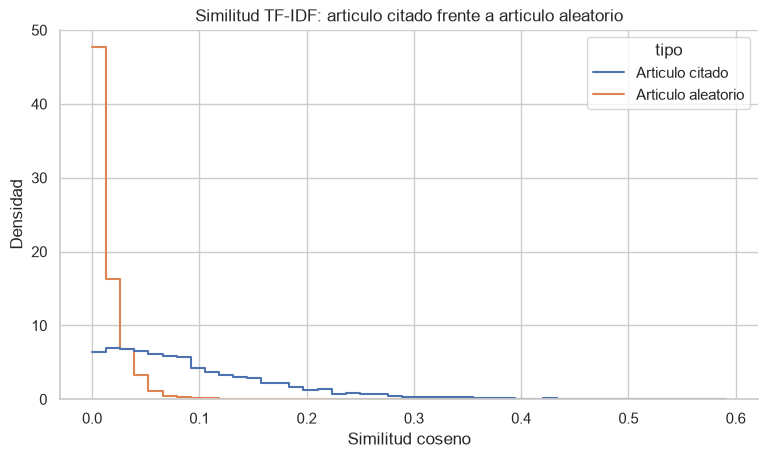
\includegraphics[width=0.68\textwidth]{eda_similitud_tfidf.png}
\caption{Similitud TF--IDF entre el contexto y el artículo citado frente a un candidato aleatorio.}
\label{fig:eda-similitud}
\end{figure}

\notabox{\textbf{Implicación para el alcance.} ACL-200 permite entrenar y evaluar la recomendación local de citas, pero no contiene las nueve etiquetas de función de cita planteadas en la propuesta de grado. Por ello, esta entrega limita el producto supervisado a relevancia y ranking; la construcción y validación humana de las etiquetas discursivas queda fuera del microproyecto.}

% ======================= 7. MAQUETA DEL PROTOTIPO =======================
\section{Maqueta del prototipo}

La interfaz inicial se dividirá en dos componentes: un recomendador de citas y un módulo de exploración del conjunto de datos. La Figura~\ref{fig:mockup} presenta la maqueta conceptual de la primera versión del prototipo.

\begin{figure}[h!]
\centering
\begin{tikzpicture}[font=\sffamily\small]

  % Outer frame
  \draw[draw=primaryblue, line width=1.2pt, rounded corners=6pt, fill=lightgray]
    (0,0) rectangle (13,7.6);

  % Title bar
  \draw[fill=primaryblue, draw=none] (0,6.9) rectangle (13,7.6);
  \node[white, font=\bfseries\sffamily] at (6.5,7.25) {LOCAL CITATION RECOMMENDER};

  % Left panel - recommender
  \draw[draw=accentblue, fill=white, rounded corners=4pt] (0.4,0.4) rectangle (6.6,6.6);
  \node[anchor=north west, color=primaryblue, font=\bfseries\footnotesize, text width=5.8cm, inner sep=1pt] at (0.6,6.45)
    {Citation context (English text)};
  \draw[draw=midgray, dashed, fill=lightgray!60, rounded corners=2pt] (0.6,4.9) rectangle (6.4,6.0);
  \node[anchor=north west, color=midgray, text width=5.5cm] at (0.75,5.85)
    {\fontsize{6.5}{8}\selectfont Write or paste the academic context where a citation is required...};

  \draw[fill=accentblue, draw=none, rounded corners=3pt] (0.6,4.35) rectangle (3.35,4.78);
  \node[white, font=\bfseries\fontsize{6.5}{8}\selectfont] at (1.975,4.565) {Recommend citations};

  \node[anchor=north west, color=primaryblue, font=\bfseries] at (0.6,3.95) {Top recommendations};
  \node[anchor=north west, align=left, font=\footnotesize] at (0.6,3.55)
    {\shortstack[l]{1. Paper A -- 0.91 \\ 2. Paper B -- 0.84 \\ 3. Paper C -- 0.76}};

  \draw[draw=midgray, fill=white, rounded corners=2pt] (0.6,0.6) rectangle (6.4,2.1);
  \node[anchor=north west, color=midgray, font=\itshape\footnotesize] at (0.75,2.0)
    {Selected paper abstract / details};

  % Right panel - dataset insights
  \draw[draw=accentblue, fill=white, rounded corners=4pt] (6.9,0.4) rectangle (12.6,6.6);
  \node[anchor=north west, color=primaryblue, font=\bfseries] at (7.1,6.35) {Dataset insights};

  \node[anchor=north west, align=left, font=\footnotesize] at (7.1,5.85)
    {\shortstack[l]{Contexts: 63,768 \\ Papers: 19,776 \\ Train / Val / Test: \\ 30,390 / 9,381 / 9,585}};

  \draw[draw=midgray, fill=lightgray!60, rounded corners=2pt] (7.1,1.2) rectangle (12.4,4.0);
  \node[anchor=center, color=midgray, font=\itshape\footnotesize, text width=4.6cm, align=center]
    at (9.75,2.9) {Charts: context length, split distribution, data quality};

\end{tikzpicture}
\caption{Maqueta inicial del tablero de recomendación local de citas}
\label{fig:mockup}
\end{figure}

% ======================= ARQUITECTURA CONCEPTUAL =======================
\section{Arquitectura conceptual del producto}

El flujo propuesto sigue una arquitectura reproducible que separa el versionamiento del código, el versionamiento de los datos, el entrenamiento y el consumo del modelo (Figura~\ref{fig:arquitectura}). Esta separación es coherente con las prácticas de MLOps orientadas a reproducibilidad y trazabilidad de los activos de aprendizaje automático (Treveil \& Dataiku Team, 2021). A la fecha de esta entrega, las dos primeras etapas del flujo --versionamiento de datos en DVC y exploración inicial-- ya están implementadas y documentadas en la Sección~\ref{sec:eda}; las etapas de entrenamiento, empaquetamiento, API y tablero se desarrollarán en las siguientes entregas del curso.

\begin{figure}[h!]
\centering
\begin{tikzpicture}[
  node distance=0.2cm,
  box/.style={draw=accentblue, fill=lightgray, rounded corners=3pt, minimum width=7.4cm, minimum height=0.68cm, align=center, text=primaryblue, font=\sffamily\footnotesize\bfseries},
  boxfinal/.style={draw=primaryblue, fill=primaryblue, rounded corners=3pt, minimum width=7.4cm, minimum height=0.68cm, align=center, text=white, font=\sffamily\footnotesize\bfseries},
  arr/.style={-{Stealth[length=2mm]}, draw=midgray, thick}
]
  \node[box] (datos) {Dataset original};
  \node[box, below=of datos] (dvc) {DVC + almacenamiento remoto};
  \node[box, below=of dvc] (prep) {Preprocesamiento y construcción de pares};
  \node[box, below=of prep] (train) {Entrenamiento y seguimiento de experimentos};
  \node[box, below=of train] (model) {Modelo seleccionado y empaquetado};
  \node[box, below=of model] (api) {API de inferencia};
  \node[box, below=of api] (dash) {Tablero interactivo};
  \node[boxfinal, below=of dash] (user) {Usuario};

  \draw[arr] (datos) -- (dvc);
  \draw[arr] (dvc) -- (prep);
  \draw[arr] (prep) -- (train);
  \draw[arr] (train) -- (model);
  \draw[arr] (model) -- (api);
  \draw[arr] (api) -- (dash);
  \draw[arr] (dash) -- (user);
\end{tikzpicture}
\caption{Arquitectura conceptual del producto}
\label{fig:arquitectura}
\end{figure}

% ======================= RESULTADO ESPERADO =======================
\section{Resultado esperado del microproyecto}

El resultado esperado es un prototipo funcional capaz de recibir un contexto académico en inglés y recomendar artículos potencialmente relevantes para citar. El análisis exploratorio de la Sección~\ref{sec:eda} confirma que el conjunto de datos es adecuado para este objetivo: la separación entre \textit{train}, \textit{validation} y \textit{test} no presenta fuga de información, y existe una señal léxica aprovechable entre el contexto y el artículo citado (90,1\,\% de las consultas evaluadas), lo que respalda TF--IDF como línea base razonable para las primeras versiones del modelo. Además del desempeño predictivo, el proyecto buscará que la solución sea reproducible y desplegable mediante versionamiento de código y datos, seguimiento de experimentos con MLflow, servicio del modelo por API, un tablero interactivo y contenerización con Docker. El prototipo permitirá demostrar el flujo completo desde la disponibilidad de los datos hasta el consumo de una predicción por parte de un usuario final.

% ======================= TRABAJO EN EQUIPO =======================
% Esta seccion se conserva dentro del reporte. La "hoja aparte" que pide la
% seccion "Entregables" de maia_pds_proy_s2.pdf se cumple con el documento
% independiente de 1 pagina `trabajo_equipo.tex`.
% \clearpage (no \newpage): primero coloca los flotantes pendientes -la
% Figura 7- y despues corta la pagina, para que esta seccion arranque sola.
\clearpage
\section{Reporte de trabajo en equipo}

El equipo distribuyó las actividades de la Entrega 1 entre la configuración de la infraestructura reproducible, la exploración de los datos, la documentación y la adecuación del reporte. Las contribuciones fueron verificadas mediante el historial de \textit{commits} del repositorio Git, de acuerdo con el requisito de evidenciar el aporte individual de cada integrante (Tabla~\ref{tab:equipo}).

\begin{table}[h!]
\centering
\caption{Aportes verificables en el repositorio}
\label{tab:equipo}
\small
\begin{tabular}{p{3.1cm} p{8.8cm}}
\toprule
\textbf{Integrante} & \textbf{Evidencia registrada} \\
\midrule
John Arias & Configuración inicial de DVC y estructura base; versionamiento del \textit{dataset}; remoto AWS S3; \textit{notebook} inicial de EDA; análisis de relaciones del \textit{dataset} e integración de contribuciones mediante \textit{Pull Request}. \\[3pt]
José Zambrana & Configuración de remoto DVC; actualización amplia del \textit{notebook} de EDA; incorporación de gráficas y evidencias; dependencias; creación y reorganización del reporte para alinearlo con la rúbrica. \\[3pt]
Carlos Caicedo & Mejoras del informe y de las evidencias DVC/S3; eliminación de contenido redundante; corrección de la maqueta; recuperación y ajuste de la arquitectura conceptual y del resultado esperado. \\[3pt]
Carlos Duque & Actualización de la documentación del proyecto mediante el \texttt{README} e incorporación de archivos asociados a la definición y reproducibilidad del entorno, incluyendo \texttt{.python-version}, \texttt{pyproject.toml} y \texttt{uv.lock}. \\
\bottomrule
\end{tabular}
\end{table}

El historial del repositorio evidencia contribuciones de los cuatro integrantes. Adicionalmente, durante la validación final se comprobó la reproducibilidad del proyecto mediante la creación de un entorno limpio, la recuperación de los datos versionados desde Amazon S3 mediante DVC y la ejecución completa del \textit{notebook} de exploración sin errores.

\section*{Referencias}
\addcontentsline{toc}{section}{Referencias}

\begin{list}{}{%
  \setlength{\leftmargin}{1.2cm}
  \setlength{\itemindent}{-1.2cm}
  \setlength{\itemsep}{10pt}
  \setlength{\parsep}{0pt}
}

\item Gu, N. (2022). \textit{Local-Citation-Recommendation} [Computer software]. GitHub. \url{https://github.com/nianlonggu/Local-Citation-Recommendation}

\item Gu, N., Gao, Y., \& Hahnloser, R.\,H.\,R. (2022). Local citation recommendation with hierarchical-attention text encoder and SciBERT-based reranking. In M. Hagen et al. (Eds.), \textit{Advances in Information Retrieval} (pp. 274--288). Springer International Publishing. \url{https://doi.org/10.1007/978-3-030-99736-6_19}

\item Treveil, M., \& Dataiku Team. (2021). \textit{Introducing MLOps: How to scale machine learning in the enterprise}. O'Reilly Media.

\end{list}

\end{document}
